\section{}

\subsection{}
A Pb–$60$ at\% Sn alloy was slowly cooled from $380^{\circ}$C to $50^{\circ}$C. Calculate the volume fraction of the primary phase at $50^{\circ}$C.

The phase diagram for an alloy of Pb and Sn is shown in figure \ref{fig:diagrama}. The temperature and composition are located in the diagram, the composition $C_0$ corresponds to a $60$\% of Sn and $40$\5 of Pb. From the figure, it can be seen that for a temperature of $50^{\circ}$C there is presence of two phases, $\alpha$ and $\beta$. From the isothermal of the temperature it is possible to obtain the values of the compositions for each phase by intersecting the ishothermal llinea with the baoundaries of the phase diagram, which gives the following results:

\begin{align*}
    C_{Sn}_{\alpha}&=4\%, & C_{Sn}_{\beta}&=99\% \\
    C_{Pb}_{\alpha}&=96\%, & C_{Pb}_{\beta}&=1\%
\end{align*}

The primary phase is the phase that has a higher fraction in the mixture, for which is necessary to calcualte the fraction of each phase, and to do that the lever rule is used. The lever rule states that the phase fraction can be calculated taking the distance of the tie line of the total composition to the border of the other phase and divide this by the total distance of the tie line \citet{callister2010materials}, as it is shown in the following equations:

\begin{align}
    \label{eq:fractions}
    W_{\alpha}&=\dfrac{C_{\beta}-C_0}{C_{\beta}-C_{\alpha}}
\end{align}

\begin{figure}[h]
    \centering
    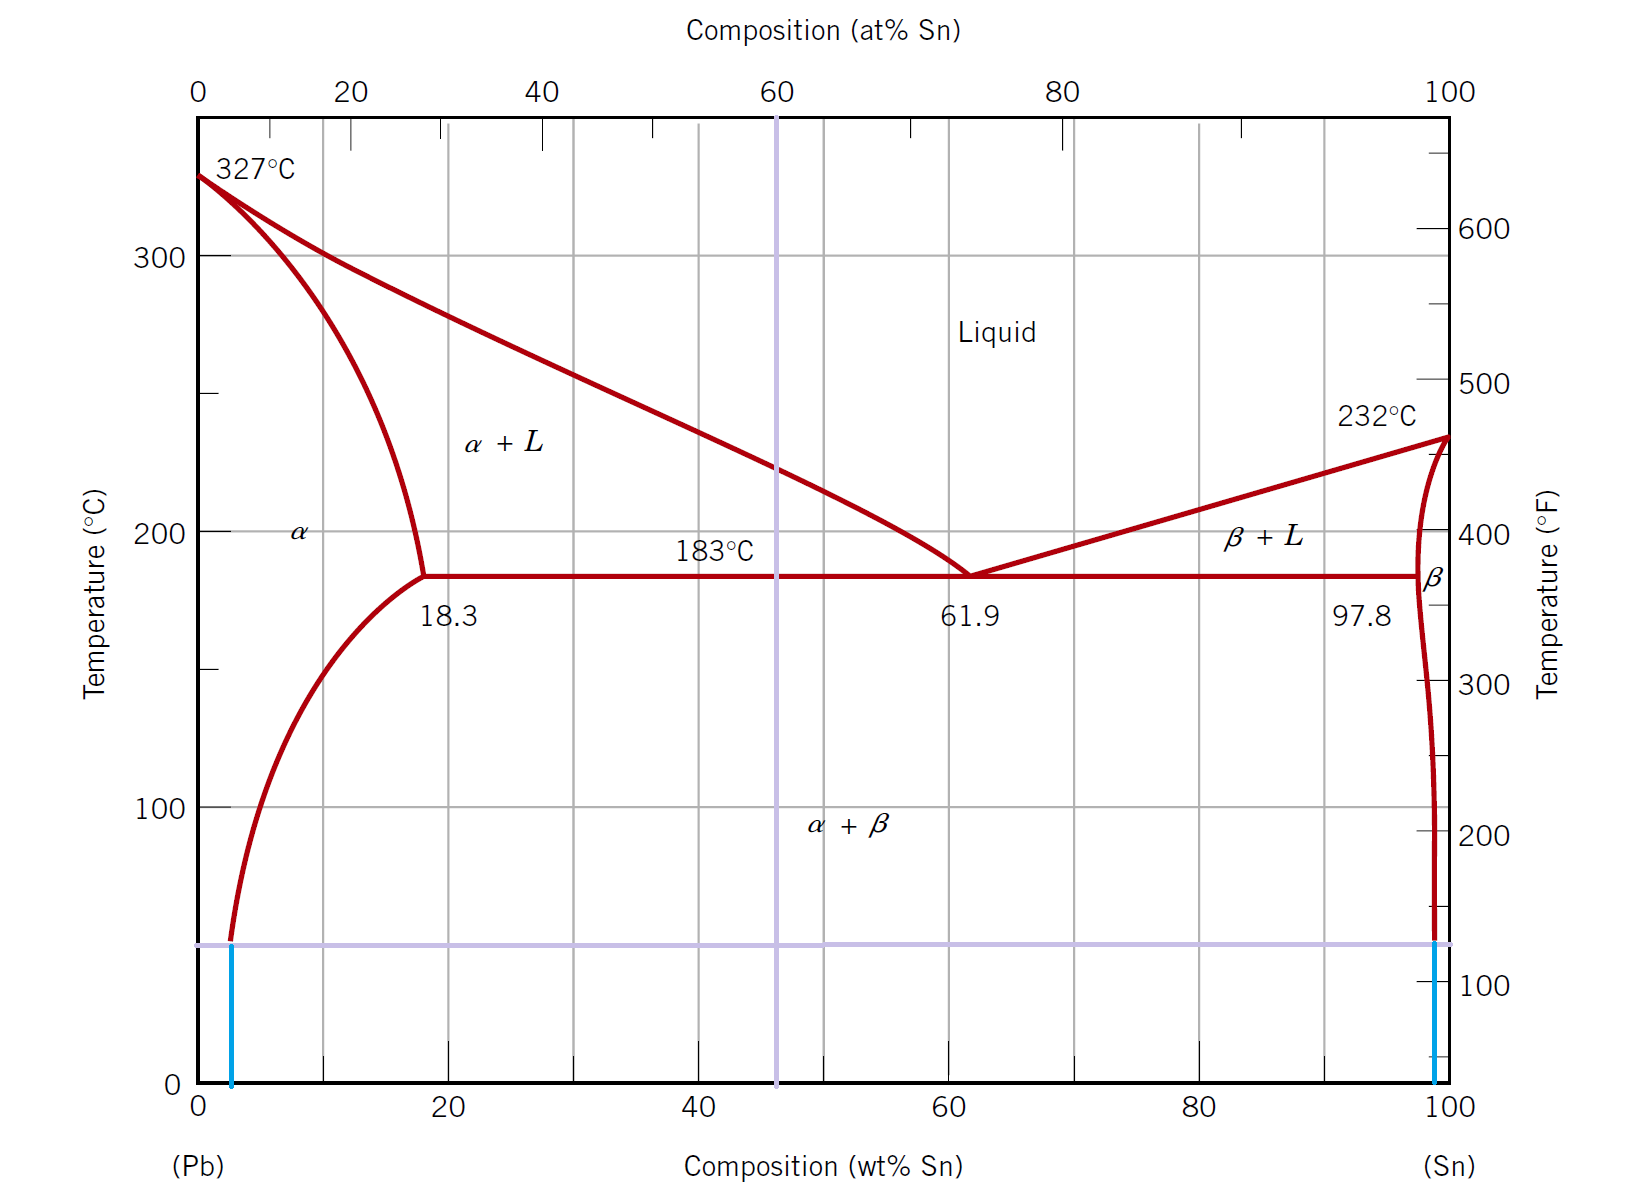
\includegraphics[width=1\textwidth]{graficas/diagrama.png}
    \caption{Phase diagram for lead-tin \\
    \textit{Source: Figure adapted from \citep{callister2010materials}}}
    \label{fig:diagrama}
\end{figure}


\subsection{}
A Pb–$25$ at$\%$ Sn alloy was slowly cooled from 380°C to 50°C. Ideally, Sn phase is expected to precipitate within Pb-phase grains, but in reality, a eutectic structure appeared. Assuming there were no experimental issues such as weighing errors, discuss the reason why this phenomenon occurred.